\documentclass[11pt,a4paper]{article}

\usepackage[T1]{fontenc}
\usepackage[utf8]{inputenc}
\usepackage{lmodern}
\usepackage[margin=25mm]{geometry}
\usepackage{microtype}
\usepackage{amsmath}
\usepackage{booktabs}
\usepackage{xcolor}
\usepackage{tikz}
\usetikzlibrary{arrows.meta,positioning}
\usepackage{enumitem}
\usepackage{hyperref}

\definecolor{navy}{HTML}{183B56}
\definecolor{bluefill}{HTML}{EAF2F8}
\definecolor{greenfill}{HTML}{EAF5EC}
\hypersetup{colorlinks=true,linkcolor=navy,urlcolor=navy,
  pdftitle={LASSQD with QCSC Prefect},
  pdfsubject={LASSQD with one node per batch using SQD's collective interface}}
\setlist{itemsep=3pt,topsep=5pt,leftmargin=*}
\setlength{\parindent}{0pt}
\setlength{\parskip}{6pt}
\setlength{\emergencystretch}{2em}
\clubpenalty=10000
\widowpenalty=10000
\newcommand{\code}[1]{\texttt{\detokenize{#1}}}
\tikzset{
  box/.style={draw=navy,rounded corners=2pt,align=center,
    font=\small,inner sep=6pt,fill=bluefill},
  worker/.style={box,fill=greenfill},
  arrow/.style={-{Stealth[length=2mm]},thick,draw=navy}
}

\title{\textbf{LASSQD with QCSC Prefect}}
\author{}
\date{}

\begin{document}
\maketitle
\vspace{-2em}

\section{The current LASSQD workflow}

LASSQD uses sample-based quantum diagonalization (SQD) to solve the fragments
of a localized active space (LAS) calculation. Quantum circuits provide samples;
classical fragment solves return reduced density matrices (RDMs), which mrh's
RDM-based LASSCF uses to update the orbitals.

The current \code{run_lassqd} driver repeats four steps:
\begin{enumerate}
  \item \textbf{Capture fragment Hamiltonians.}
  \code{fragment_hamiltonians} enters mrh with temporary callbacks that collect
  the Hamiltonians instead of solving them. Once all inputs are captured,
  execution stops before the orbital update.
  \item \textbf{Prepare and sample circuits.}
  A caller-supplied builder prepares each fragment's circuit in its ROHF basis.
  The driver optionally places the circuits side by side, transpiles them,
  and submits one sampler job. It waits for all counts before continuing.
  \item \textbf{Solve fragments.}
  The driver installs \code{FragmentSQD} callbacks and enters mrh again.
  mrh repeats its integral and embedding preparation, then calls the solvers
  sequentially. Each solver performs configuration recovery and batched
  selected-CI solves, returning the lowest-energy batch's energy and RDMs
  across recovery rounds. Determinants can carry over between rounds and cycles.
  \item \textbf{Update orbitals.}
  mrh computes the coupled LAS energy and takes one orbital macrostep.
  The driver repeats until the absolute total-energy change is below the
  tolerance or the cycle limit is reached.
\end{enumerate}

The two mrh calls repeat Hamiltonian preparation; the SQD solves run only in
the second call. Circuit preparation and SQD also independently compute the
fragment ROHF basis. The driver has no distributed scheduling or complete
restart contract: \code{FragmentSQD.output_dir} omits the previous-basis and
random-generator state needed for continuation.

\section{The proposed LASSQD--QCSC Prefect distributed workflow}

The design uses \textbf{mrh unchanged}. LASSQD captures the fragment
Hamiltonians, solves the fragments outside mrh, then re-enters mrh with
callbacks that return the completed results. Prefect coordinates dependencies;
QCSC launches HPC jobs and handles QPU submission and fetching.

The selected scope is several fragments, with each diagonalization batch
fitting on one node. For fragment $f$ with $B_f$ batches, launch one MPI job on
$B_f$ nodes, with one rank per node and one batch per rank. Retain that
allocation across recovery rounds. Different fragments use separate MPI jobs
and can run concurrently. Use the existing collective
\code{diagonalize_fermionic_hamiltonian} interface with an application-supplied
\code{sci_solver}; SQD's recovery loop remains unchanged.

The Prefect coordinator exchanges storage references. Full numerical arrays
and CI vectors remain on HPC, including MPI transfers between the ranks of
each fragment job. The control rank must accommodate gathered batch results;
the memory requirements below are stronger than one batch fitting on one node.

Figure~\ref{fig:distributed-workflow} shows the complete workflow and the
execution nodes. Node labels denote resource roles: short HPC stages may reuse
nodes, and the coordinator, scheduler submitter, and QPU gateway may share a
service host. Each fragment's MPI allocation has $B_f$ distinct compute nodes.

\begin{figure}[htbp]
\centering
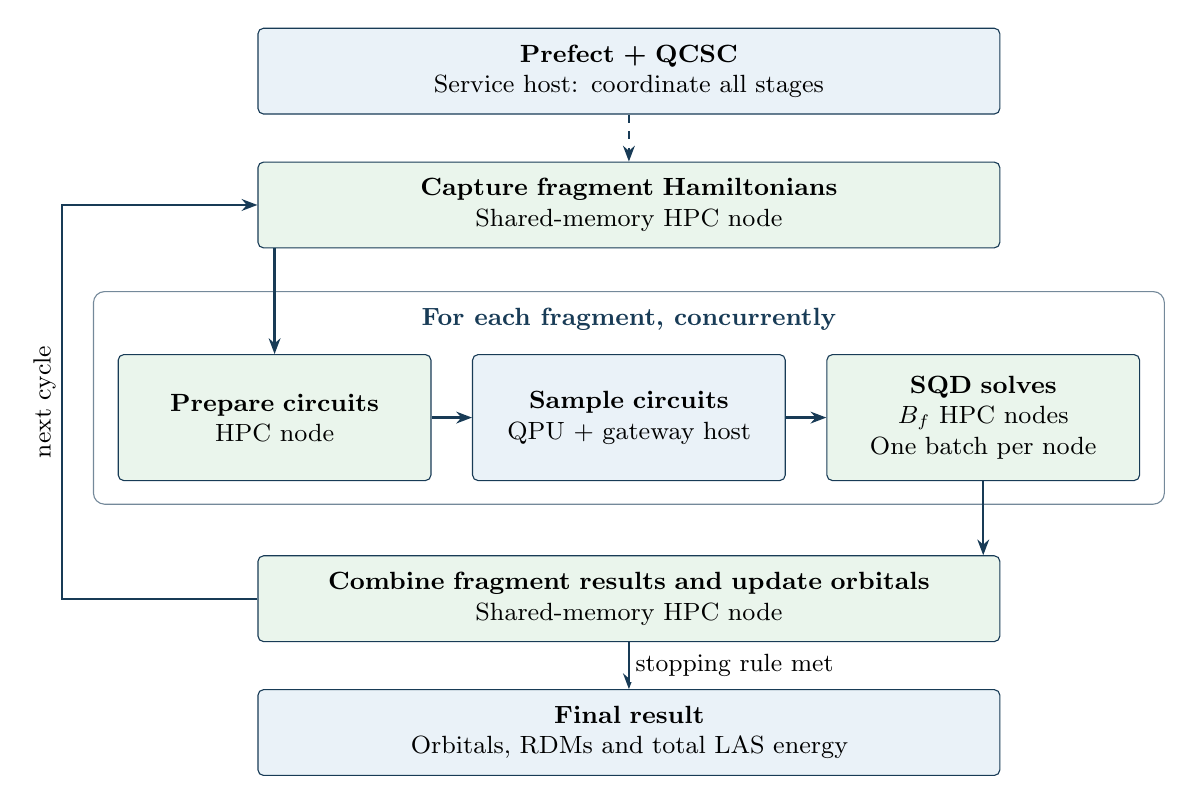
\begin{tikzpicture}[
  stage/.style={worker,text width=9cm,minimum height=1.05cm},
  fragmentstage/.style={box,text width=3.55cm,minimum height=1.6cm},
  flowlabel/.style={font=\small,fill=white,inner sep=2pt}
]
  \node[stage,fill=bluefill] (coordinator) at (0,0)
    {\textbf{Prefect + QCSC}\\Service host: coordinate all stages};
  \node[stage] (capture) at (0,-1.7)
    {\textbf{Capture fragment Hamiltonians}\\Shared-memory HPC node};
  \draw[arrow,dashed] (coordinator) -- (capture);

  \draw[draw=navy!60,rounded corners=4pt]
    (-6.8,-2.8) rectangle (6.8,-5.5);
  \node[font=\small\bfseries,text=navy] at (0,-3.15)
    {For each fragment, concurrently};
  \node[fragmentstage,fill=greenfill] (prepare) at (-4.5,-4.4)
    {\textbf{Prepare circuits}\\HPC node};
  \node[fragmentstage] (sample) at (0,-4.4)
    {\textbf{Sample circuits}\\QPU + gateway host};
  \node[fragmentstage,fill=greenfill] (solve) at (4.5,-4.4)
    {\textbf{SQD solves}\\$B_f$ HPC nodes\\One batch per node};
  \draw[arrow] (capture.south -| prepare.north) -- (prepare.north);
  \draw[arrow] (prepare) -- (sample);
  \draw[arrow] (sample) -- (solve);

  \node[stage] (update) at (0,-6.7)
    {\textbf{Combine fragment results and update orbitals}\\Shared-memory HPC node};
  \draw[arrow] (solve.south) -- (update.north -| solve.south);
  \node[stage,fill=bluefill] (done) at (0,-8.4)
    {\textbf{Final result}\\Orbitals, RDMs and total LAS energy};
  \draw[arrow] (update) -- node[flowlabel,right] {stopping rule met} (done);
  \draw[arrow] (update.west) -- (-7.2,-6.7)
    -- node[flowlabel,rotate=90,above] {next cycle}
    (-7.2,-1.7) -- (capture.west);
\end{tikzpicture}
\caption{Workflow and node roles. Each fragment uses one MPI job with one
rank per node; recovery rounds stay within that job. The orbital update waits
for all fragments. Repeat until energy convergence or the cycle limit.}
\label{fig:distributed-workflow}
\end{figure}

\textbf{Capture a fixed embedding.}
An HPC task restores a committed snapshot of orbitals and fragment RDMs.
It passes those RDMs explicitly to mrh and captures all fragment Hamiltonians
through temporary callbacks. mrh constructs their effective one-electron
Hamiltonians before its fragment loop, so the captured problems can be solved
concurrently without changing that dependency structure.

\textbf{Run fragment workflows concurrently.}
Each fragment prepares its ROHF basis and transformed integrals once, sharing
them between circuit construction and SQD. Circuit preparation runs on HPC;
a QPU gateway obtains and stores counts. SQD can start as soon as that
fragment's counts arrive, although a shared QPU may serialize sampling.
Reserve the multi-node solve allocation only after the counts are available.
Short circuit-preparation stages can be bundled to reduce queue overhead.

\textbf{Use SQD's collective interface within each fragment.}
Rank 0 restores the fragment checkpoint, including carryover and its basis,
and prepares the resolved SQD inputs. Broadcast the integrals, counts, basis
data, numerical options, included configurations, and starting random-generator
state so all ranks enter SQD with agreeing arguments. Every rank calls
\code{diagonalize_fermionic_hamiltonian}. Within each recovery round:
\begin{enumerate}
  \item SQD performs recovery and subsampling on rank 0 and broadcasts the
  ordered list of determinant batches to all ranks.
  \item All ranks enter the custom \code{sci_solver}. Rank $r$ solves batch
  index $r$ locally using Fulqrum or PySCF and the threads assigned to its node.
  Rank 0 also solves its batch. Each rank owns its numerical solver objects.
  \item The adapter gathers the full \code{SCIResult} objects on rank 0 and
  returns them there in the original batch order. Other ranks may return an
  empty list: only rank 0 consumes the adapter's results in the inspected SQD
  implementation. These are ordinary states containing full CI amplitudes.
  \item SQD invokes the callback on rank 0, selects the round's best batch,
  checks convergence, and updates occupancies and carryover there. It
  broadcasts the iteration state, including the best-so-far and current
  \code{SCIResult} objects, to every rank.
\end{enumerate}
This gather and broadcast synchronizes successive rounds. Fragments advance
independently; a slow batch delays its own fragment's next round. The final
best result is available on every rank. Only rank 0 performs LASSQD's final
carryover extraction, RDM construction and basis rotation, and checkpoint and
manifest writes. SQD guards its own callback, but does not guard these
operations in today's \code{FragmentSQD} wrapper.

Each fragment returns energy including the constant Hamiltonian term,
spin-resolved 1-RDMs of shape $(2,n_f,n_f)$, and a spin-summed 2-RDM of shape
$(n_f,n_f,n_f,n_f)$. The RDMs must use the original LAS fragment basis.
Store these arrays and the fragment continuation state under references;
CI vectors need not pass through the Prefect coordinator.

\textbf{Replay mrh and commit the orbital update.}
Wait for all required fragment results, then restore the original snapshot.
Re-enter mrh with callbacks that validate each requested Hamiltonian against
the captured input and return the stored energy and RDMs. Pass the
\emph{original starting RDMs} to the kernel; the callbacks introduce the new
RDMs at the solve boundary. Use \code{max_cycle_macro=1} and
\code{max_cycle_rdmjk=0}, as in the current driver.

mrh repeats global preparation and visits the callbacks sequentially, but no
SQD solve is repeated. It then performs the coupled energy calculation, orbital
update, and canonicalization. Commit the returned orbitals and RDMs together
in their consistent basis. Embedded fragment energies are not simply additive:
the total LAS energy includes interfragment contributions.

\textbf{Launch jobs through QCSC.}
A LASSQD worker executable reads a stage request and writes a validated result
manifest. The flow invokes it through \code{run_job_from_blocks}, using
\code{CommandBlock} for the executable, \code{ExecutionProfileBlock} for
resources, and \code{HPCProfileBlock} for site configuration. Schedule capture,
fragment preparation, and replay as classical HPC stages. For each collective
fragment solve set \code{num_nodes} to $B_f$, \code{mpiprocs=1}, an MPI-capable
launcher, and appropriate \code{ompthreads} and BLAS/OpenMP environment
settings. Configure the site's launcher and placement options explicitly;
on Slurm the total task count must also agree with $B_f$. On Fugaku the PJM
and launcher MPI options must express the same rank layout.

At startup verify that there are $B_f$ ranks on $B_f$ distinct nodes and that
SQD detects the same MPI rank and size as \code{MPI.COMM_WORLD}. The inspected
SQD detects MPI at import time from launcher environment variables. Each
fragment gets its own MPI world; its ranks all participate in the same SQD
call. Make MPI calls from the main thread, with an appropriate MPI thread
support level, while the local numerical libraries use node-local threads.

Use stable fragment-job keys and QCSC's registry-backed submit/monitor APIs
for restartable scheduling. \code{run_jobs_from_blocks_bulk} can manage a
pool of complete fragment MPI jobs; individual diagonalization batches remain
inside their fragment allocation. Fugaku's \code{GlobalFugakuBulkRunner}
supports rolling progress as fragment counts arrive. Other scheduler targets
need an explicit queue probe for bulk execution. Bound both active fragment
jobs and the total reserved nodes $\sum_f B_f$; a job-count limit alone does
not impose a node budget. The simple \code{run_job_from_blocks} path remains
useful for initial local and scheduler validation.
The submitter needs scheduler access and shared storage or explicit file staging.

The gateway awaits QCSC's asynchronous \code{QCSCSamplerV2} submission and
fetching, saving provider job references and counts durably. It cannot be
substituted directly into today's synchronous driver. Circuit grouping remains
configurable so fragments can obtain counts independently where useful.

\textbf{Persist enough state to restart.}
Requests identify the parent snapshot, fragment, Hamiltonian, basis, acquisition,
and numerical settings. Save counts, carryover strings and their basis, and each
fragment's full random-generator state. Assign independent streams to sampling
and each fragment: the current notebook shares one generator, whose serial
draw order cannot simply be carried into concurrent execution. Use the same
stream policy in the serial reference. During collective SQD, rank 0 owns the
advancing recovery RNG; its saved state is authoritative. Give any stochastic
local eigensolver a seed tied to the logical batch, not completion order.

Treat a failed collective fragment solve as one failed MPI job. Propagate
errors or abort the MPI world so peers cannot remain blocked in a collective,
including failures in rank-0 preparation, callbacks, and finalization.
The initial restart contract reruns the whole fragment call from its input
checkpoint and saved counts; the current SQD API does not expose complete
mid-round continuation state. Preserve completed results from other fragments.

Persist scheduler and QPU job references and reconcile ambiguous submissions
before retrying. Check scheduler exit status as well as result validity. Publish
the result manifest atomically only after all referenced files are complete and
validated; QCSC's expected-output check alone tests file existence. Handle
deferred submissions explicitly when using the rolling Fugaku runner. Commit
a new global state only after replay and the orbital update succeed.

\section{Implementation outline}

Implement the workflow within this repository's existing \code{lassqd}
package, including optional modules for QCSC workflows. Use SQD's existing
collective interface to distribute one batch per node within each fragment
job. Both the local solves and the collective result aggregation must fit
their assigned resources. The inspected upstream libraries need no source
changes; the optional mrh optimization is a separate follow-up.

In \code{lassqd/hybrid.py}, separate capture, circuit preparation, sampling,
fragment solving, and replay into callable stages. Retain a local driver
composed from the same stages. In \code{lassqd/las.py}, pass explicit
\code{casdm1frs}/\code{casdm2fr}, restore the same snapshot for replay, and
validate Hamiltonians before supplying cached results. These RDM arguments
already exist in mrh; passing them avoids repeated implicit CI/CSF initialization.
Add validation and checkpoint/restore for the global orbitals and fragment
RDMs as one consistent state.

In \code{lassqd/basis.py} and \code{lassqd/sqd.py}, share prepared basis data
between circuit construction and SQD. Add checkpoint/restore for carryover,
\code{prev_mo}, resolved solver options, and random-generator state.
Separate rank-0 input preparation and finalization from the SQD call that every
rank must enter. Keep CI-dependent processing inside the fragment MPI job and
make expensive diagnostics configurable: today's callback computes
\code{spin_square()} for every batch on rank 0.

Implement the collective adapter in LASSQD. Check the
batch count against the MPI world size, solve exactly one assigned batch on
each rank, and gather results in batch order. Preserve the existing energy,
spin, determinant-ordering, and RDM conventions. The Fulqrum adapter must
retain the transpose between Fulqrum's vector ordering and SQD's
alpha-by-beta amplitude matrix. Each rank can reuse its own prepared operator
across recovery rounds at fixed fragment integrals. Configure a serial
adapter with the same local solver to provide the numerical reference.

Define versioned request/result records with array references. Place Prefect
flows, worker entry points, the QPU gateway, storage adapters, MPI resource
profiles, and failure/retry handling in optional modules within the existing
\code{lassqd} package, with QCSC and MPI dependencies provided as extras.
Co-installation with the inspected
QCSC packages requires Python 3.11 or newer; separate gateway and worker
environments can communicate through the records. The MPI worker environment
also needs \code{mpi4py} built for the site's MPI runtime and an SQD revision
with the inspected collective implementation. LASSQD's current
\code{qiskit-addon-sqd>=0.12.0} dependency alone does not ensure this capability.

\subsection*{Resource limits and validation}

Size each node for its batch's determinant space, projected Hamiltonian,
eigensolver workspace, integrals, and local result. Rank 0 additionally gathers
all $B_f$ results, including their full CI states and any supplied RDMs, while
retaining earlier iteration state. Every rank receives the broadcast best and
current results. Account for serialization buffers and temporary copies.
Consequently, \emph{one batch fitting on a node is necessary but insufficient}
for this unchanged-interface design. Benchmark the gather/broadcast memory
peak as well as the local eigensolve. The design retains local CI storage
and replicated iteration results.

Control BLAS/OpenMP threads within each node and verify rank placement.
Global capture and replay use mrh's existing numerical execution; provision a
suitable shared-memory node for their integrals and orbital calculations.
Dense 2-RDM storage grows as $n_f^4$. Requesting additional nodes does not
distribute those arrays: the parallelism comes from independent batch solves.
Retaining fragment allocations avoids queueing between recovery rounds, but
nodes wait during rank-0 recovery, diagnostics, and result aggregation, and for
the slowest batch in each round. Measure these costs before claiming an optimal
node count or speedup.

First build a serial capture/replay reference, then compare the collective
adapter using identical counts, ordered batches, local solver settings, and
initial random states. Test multiple ranks locally before verifying one rank
per node on the target scheduler. Exercise QCSC's local target separately for
the worker request/result protocol. Check energies, RDM conventions, basis
consistency, carryover, and root-owned RNG continuation across multiple rounds
and hybrid cycles. Inject failures on both rank 0 and another rank to verify
termination, whole-fragment restart, and the absence of partial commits.
Measure repeated preparation, queue time, local solves, communication,
rank-0 processing, orbital work, and peak memory on every rank.

Validate explicit RDM initialization separately because it can change today's
trajectory. Preserve the current use of \code{h1s[0]} for fragment problems and
the energy-change stopping rule during the execution refactor. Full
spin-dependent embedding and stronger convergence criteria are separate
numerical changes.

\section{Optional follow-up: changes to mrh}

The workflow above requires no mrh changes. A separate optimization can replace
capture/replay with public numerical stages:
\begin{itemize}
  \item \code{prepare_las_iteration} builds fragment Hamiltonians and retains
  the global integral and embedding intermediates.
  \item \code{advance_las_orbitals} consumes completed fragment RDMs, reuses
  those intermediates, and performs the orbital update without invoking
  fragment solvers.
\end{itemize}

These interfaces remove the second initial preparation pass. Integral
transformations required by changed orbitals still occur. The extension does
not change the Prefect task graph or make mrh responsible for parallel workers.
Adoption belongs after validation and profiling of the unchanged-mrh workflow;
compare its energies, orbitals, and RDMs against that capture/replay reference.

\section{Inspected source revisions}

The design above is a proposal based on the following local source revisions.
The application collective adapter and distributed driver remain to be
implemented and validated; MPI performance has not been measured here.

\begin{center}
\small
\begin{tabular}{@{}ll@{}}
\toprule
Repository & Inspected commit \\
\midrule
LASSQD (code before this report update) & \code{14f4c32b57ce} \\
Qiskit addon SQD & \code{8124d790600a} \\
Fulqrum & \code{8ed62cf8d142} \\
QCSC Prefect & \code{d9e63289686a} \\
mrh & \code{f007765830b6} \\
\bottomrule
\end{tabular}
\end{center}

The key source interfaces are:
\begin{itemize}
  \raggedright
  \item SQD: \path{qiskit_addon_sqd/fermion.py}, particularly
  \code{diagonalize_fermionic_hamiltonian}, \code{_IterationState}, and
  \code{solve_sci_batch}; MPI detection and broadcasts in
  \path{qiskit_addon_sqd/processes.py}.
  \item LASSQD: \path{lassqd/las.py}, \path{lassqd/hybrid.py},
  \path{lassqd/sqd.py}, and the Fulqrum adapter in \path{docs/lassqd.ipynb}.
  \item mrh: \path{my_pyscf/mcscf/lasscf_rdm.py} and
  \path{my_pyscf/mcscf/lasscf_sync_o0.py}, for the RDM kernel and fixed-embedding
  fragment loop.
  \item QCSC: \path{packages/qcsc-prefect-executor/src/qcsc_prefect_executor/from_blocks.py},
  the executor's \path{bulk/} package, and \path{docs/howto/howto_use_bulk_hpc_jobs.md};
  native Qiskit wrappers in
  \path{packages/qcsc-prefect-qiskit/src/qcsc_prefect/integrations/qiskit/wrappers.py}.
  \item Fulqrum: \path{fulqrum/core/linear_operator.py}, for the local projected
  Hamiltonian and its mutable subspace, and \path{fulqrum/core/spmv.pyx}.
\end{itemize}

\end{document}
